\documentclass[english, a4paper, 12pt]{article}

\usepackage[T1]{fontenc}
\usepackage[utf8]{inputenc}
\usepackage{amsmath}
\usepackage{titlepic}
\usepackage{amssymb}
\usepackage{amsfonts}
\usepackage{babel}
\usepackage{enumerate}
\usepackage{color}
\usepackage{wrapfig}
\usepackage{fancyhdr}
\usepackage{subfig}
\usepackage{mhchem} % Package for chemical equation typesetting
\usepackage{graphicx} % Required for the inclusion of images
\usepackage[left=1.0in, right=1.0in, top=0.75in, bottom=0.75in]{geometry}
\usepackage{float}
\newcommand{\tab}{\hspace*{2em}}
\setlength\parindent{0pt} % Removes all indentation from paragraphs
\newcommand{\horrule}[1]{\rule{\linewidth}{#1}} 

\title{ 
\includegraphics[scale=0.5]{fctuc.jpg}\\
		\bigskip\bigskip\bigskip\bigskip
		\horrule{3.5pt}		
		\LARGE Department of Informatics Engineering\\\medskip
		\Large Master in Informatics Engineering\\\medskip
		\Large Pattern Recognition Techniques\\\medskip
		\large 2013/2014\\\bigskip\horrule{2.5pt}\bigskip\bigskip
		}

\date{}	
		
		
\begin{document}
\begin{titlepage}

\clearpage
\maketitle
\thispagestyle{empty}


\begin{center}
		\Huge \textcolor{blue}{{\bf Event Matching System(EMS)}} \\
\end{center}
\vfill
\begin{center}
		\author{	
			\large Celso Rafael Clara Mendes\\
			\large celsom@student.dei.uc.pt\\
			\large 2009109378\bigskip\medskip\\
			\large Igor Nelson Garrido Cruz\\
			\large igorcruz@student.dei.uc.pt\\
			\large 2009111924
		}
\end{center}
\end{titlepage}


\newpage
\thispagestyle{empty}
\tableofcontents

%%%%% Indice
%\voffset=-2cm

%\clearpage
%{\it texto italico}

%----------------------------------------------------------------------------------------
%	SECTION 0
%----------------------------------------------------------------------------------------
\newpage
\setcounter{page}{1}
\section{Introduction}
\tab In the present work we intend to implement and analyze an Event Matching System (EMS).\smallskip\\
\tab With the introduction of new Information and Communication technologies and the proliferation of the internet access and social media, "big data" databases are everyday more common. However it is hard to extract meaning from these databases for intelligent usage, in other words it is hard to attain semantic information from the "big data". In this work we implement an EMT system that could operate in such systems in order to verify if two events are the same or not.\smallskip\\
\tab For that we used a real dataset consisting of 2090 pairs of events from the south-Asian country of Singapore labeled as matches/non-matches. For each event you are given the following characteristics: event identifier, event title, venue, start/end dates and times, address, latitude, longitude, categories and description.\smallskip\\
\tab We are going to study diverse methods of feature selection, different classifiers (Bayes, SVM, Fisher, k-NN), data sampling techniques and evaluation metrics to analyze machine learning technologies applies to EMS.\\
\tab With the diverse classifiers and features studied we are going to develop a Matlab GUI which allows the user to easily test diverse machine learning techniques that can be applied to the problem. \smallskip\\
\pagebreak


%----------------------------------------------------------------------------------------
%	SECTION 1
%----------------------------------------------------------------------------------------
\section{Pre-Processing and Feature Extraction}
\tab The event's data is not directly usable for Pattern Recognition as it is available in the dataset. The dataset is made of text, which are not directly usable by classifiers.
In order to overcome this issue we used a python script which extract numerical data from the raw text.\\

\tab  {\bf Distance between characters - }We implemented a count of occurrences of characters in each string and then calculated the distance between each count doing the sum of the absolute values of the subtraction of the occurrences. This measure is then divided by the maximum sum of characters between both strings, approximating to 0 if both strings tend to be equal or 1 if the characters are completely different. If both strings are empty we manually set this distance to be zero.\medskip\\

\tab {\bf Levenshtein's Distance - }The Levenshtein distance between two words is the minimum number of single-character edits (insertion, deletion, substitution) required to change one word into the other. This distance was calculated with the Fuzzycomp Python's library.\medskip\\

\tab  {\bf Jaccard's Distance - }The Jaccard similarity coefficient is a statistic used for comparing the similarity and diversity of the sample sets, in this case two strings. The Jaccard coefficient measures similarity between sample sets, and is defined as the size of the intersection divided by the size of the union of the sample sets. This distance was calculated with the Fuzzycomp Python's library.\medskip\\

\tab  {\bf Jaro's characters - } The Jaro distance metric is designed and best suited for short strings such as person names. The higher the Jaro distance for two strings is, the more similar the strings are (0 - no similarity, 1 - same string).  This distance was calculated with the Fuzzycomp Python's library.
\medskip\\

\bigskip
{\bf Title's Features:}\medskip\\
\tab  All the punctuation was removed from the strings.\\
\tab  Multiple white-spaces were reduced to a single one.\\
\tab  Distance between characters;\\
\tab  Levenshtein Distance;\\
\tab  Jaccard Distance;\\
\tab  Jaro Distance.\medskip\\

{\bf Venue's Features:}\medskip\\
\tab  All the punctuation was removed from the strings.\\
\tab  Multiple white-spaces were reduced to a single one.\\
\tab  If some venue is empty we use the character '-' to represent it.\\
\tab  Distance between characters;\\
\tab  Levenshtein Distance;\\
\tab  Jaccard Distance;\\
\tab  Jaro Distance.\medskip\\

\pagebreak
{\bf Starting Time's Features:}\medskip\\
\tab  All the punctuation was removed from the strings.\\
\tab  Times were converted to integers.\\
\tab  Subtraction between starting time of events was extracted.\medskip\\

{\bf Distance's Features:}\medskip\\
\tab  To extract distances between events we used the euclidean distance.\medskip\\

{\bf Categories Features:}\medskip\\
\tab  To extract features from the categories we used regular expressions to capture the text inside parenthesis and then we removed punctuation and invalid text.\\
\tab  After that we create a list of categories of each instance and we calculate the minimum Levenshtein's distance between all of the categories of each event.
\medskip\\

{\bf Description Features:}\medskip\\
\tab  To extract features from the description we remove punctuation, and we make a list of words.\\
\tab  Then we check how many of the words are common to both of the descriptions and divide by the maximum number of words, giving us a relative measure of much of the description is common to both events.
\medskip\\

%----------------------------------------------------------------------------------------
%	SECTION 2
%----------------------------------------------------------------------------------------
\section{Feature Selection}
\tab Feature selection is an important pre-processing step for solving machine learning problems. A good feature selection method may not only improve the performance of the final classifier, but also reduce the computational complexity of it.\\
\tab We used multiple methods to implement feature selection. In this chapter we will present our studies and a make some comments on our thoughts.
\subsection{Principal Component Analysis (PCA)}
\tab PCA was invented in 1901 by Karl Pearson. The method is mostly used as a tool in exploratory data analysis and for making predictive models.In the context of machine learning, PCA is a method of analysis which involves finding the linear combination of a set of variables that has maximum variance and removing its effect by reducing the dimensionality. By other words it is is a statistical procedure that uses orthogonal transformation to convert a set of observations of possibly correlated variables into a set of values of linearly uncorrelated variables called principal components.\\
\tab PCA was implemented in our work as a method of transforming the features obtaining new ones as projections.
\subsection{Kruskall-Wallis}
\tab The Kruskall-Wallis assesses whether c independent samples are from the same population (or from populations with continuous distribution) and from the same median for the variable being tested.
In order to choose the most discrimative features we should choose the ones with a higher variance given by Chi-Square.

\tab We tested the features given by the default extraction and the features after applying Principal Component Analisys (PCA).
Looking at the values, the raw data seems to be more  discriminative.\bigskip\\

\begin{figure}[H]
  \centering
  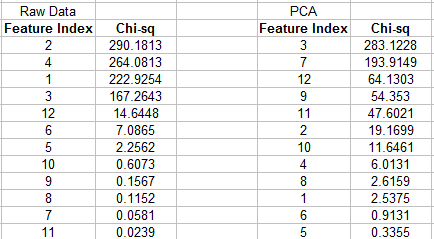
\includegraphics[scale= .8]{kruskallwallis.png}
  \caption {Kruskall-Wallis test results for raw data and for features after PCA 	projection.}
\end{figure}
\bigskip
\begin{figure}[H]
  \centering
  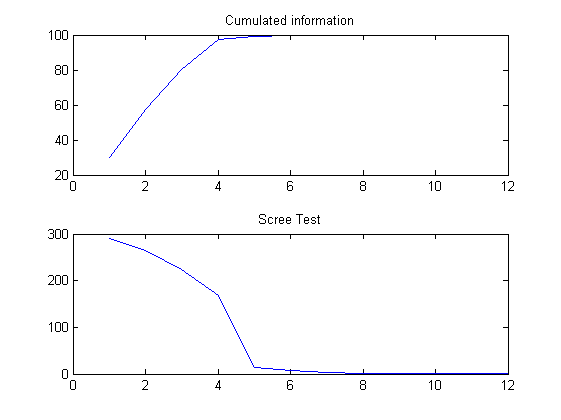
\includegraphics[scale= .8]{no_pca_features_information.png}
  \caption {Feature tests for raw data}
\end{figure}

\begin{figure}[H]
  \centering
  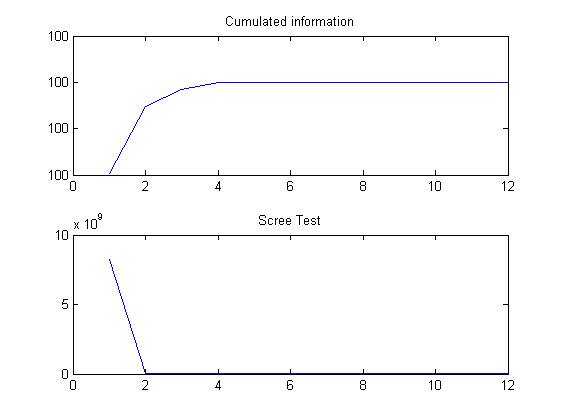
\includegraphics[scale= .8]{pca_features_information.png}
  \caption {Feature tests for PCA data}
\end{figure}
\tab As we can see in the upper plots ,using Kaiser Test, Scree Tests and Visual Threshold, without PCA the number of features that we should use to build the classifier should be around 5, since with less than that we lose too much information and with more than that we have too much dimensionality for the classifier to learn and generalize. With PCA the optimal number tends to be a little lower, decaying to 3 or 4 features. 

\subsection{Area under Curve (AUC)}
\tab The AUC can also be used as a feature selection method. In the project we used it to plot the sensibility over the specificity of each feature. After that the features are sorted by descent values of AUC and we select the highest AUC N features.\\
\begin{figure}[H]
  \centering
  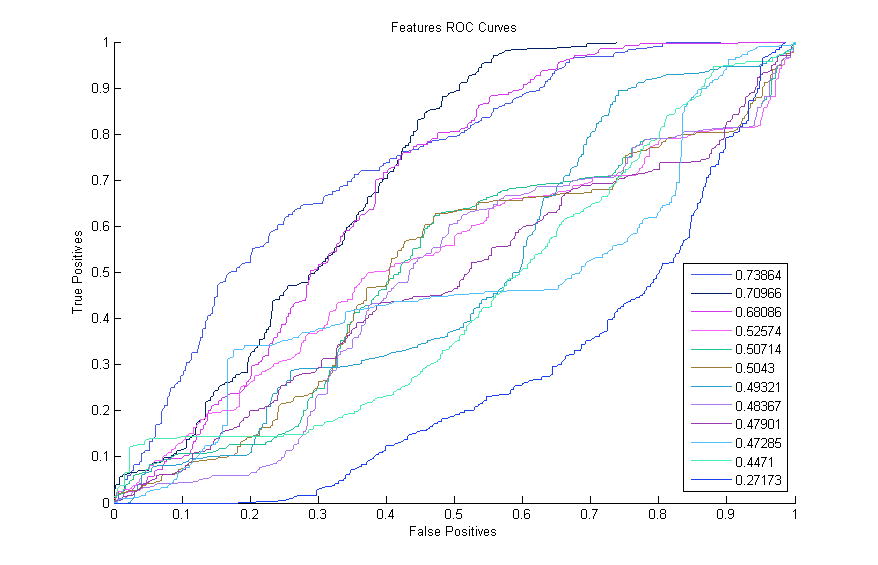
\includegraphics[scale= 0.5]{froc.png}
  \caption {ROC Curves for feature extraction}
\end{figure}
\tab Analysing the figure 4 we can see that some features are obviously more discriminant than others. To each feature is assigned an index and we proceed to the sort of features by descent. With this approach we make sure that when the user selects N features we can provide the best N features in terms of AUC of the ROC curve.
%----------------------------------------------------------------------------------------
%	SECTION 3
%----------------------------------------------------------------------------------------
\section{Data Sampling}
\tab For data sampling we implemented a 3 different methods of evaluating the classifier.
\subsection{Hold-out}
\tab For the hold-out method of validation we subdivided all the dataset in two parts. The first part (80\%) of the total number of data was used to train the classifier. The second part (20\%) was used to evaluate the classifier.\\
\tab This kind of evaluation is more reliable than using the same data to train and test. In fact the usage of different sub-sets allows the user to have a better insight of the performance of the classifier since the data used to test is independent than the data used to train. This approach gives us a better metric to evaluate if the algorithm is making the correct generalizations and learning the correct weights that need to be stablish related to the data.\\
\tab Although being better than using the same dataset to train and test, the hold-out method is not as precise as the cross-validation since it is more susceptible of noises and statistical variances of data of the patterns in the dataset. 
\subsection{Cross-Validation}
\tab For validation of the classifiers created in the project we used k-fold cross validation. This method allows us to generalize how the classifier will perform in an independent dataset. On each round of the cross-validation we partition the input data into two complementary subsets, the training set and the validation set. Then the classifier is trained with the training set and validated with the validation set. In order to achieve more consistent results and reduce its variability, multiple rounds are used splitting the dataset into different partitions and the final result is the average of each round.\\
\subsection{Bootstrap}
\tab Using the bootstrap method to create a training set method, we take patterns of our dataset and make a random choice of its elements allowing for repetition. In our implementation the test set is our original full dataset, thus making our implementation the 'simple error bootstrap'.\\
\tab With this method of date sampling we got better results when comparing with the previous two methods, this is due to the fact that we are using several training sets, so there is a wide variety of data, and using the mean of the performance metrics to join the classifiers performance metrics, we also get more stable results.

%----------------------------------------------------------------------------------------
%	SECTION 4
%----------------------------------------------------------------------------------------
\pagebreak
\section{Classifiers}
\tab The classifiers implemented for this work were the Bayes, K-NN, Fisher and SVM.

\subsection{Bayes}
\tab Bayes classifiers are probabilistic classifiers based on the Bayes' theorem. \smallskip\\
\tab We used the Maximal Likelihood estimation of Gaussian mixture model for implementing the Bayes classifier. This classifier minimizes the Bayesian risk of loss. The input vectors X are classified into classes with the highest {\it a posterior} probability computed from given model.\smallskip\\

\begin{figure}[H]
	\centering
	\begin{minipage}[b]{0.45\linewidth}
		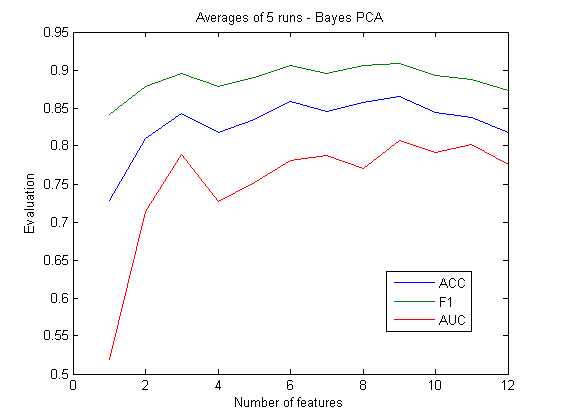
\includegraphics[scale= 0.5]{bayes_pca.png}
		\caption{Bayes PCA}
		\label{fig:minipage1}
	\end{minipage}
	\quad
	\begin{minipage}[b]{0.45\linewidth}
		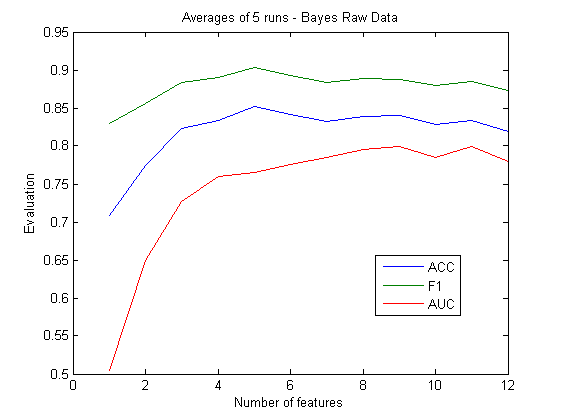
\includegraphics[scale= 0.5]{bayes_raw_data.png}
		\caption{Bayes RAW data}
		\label{fig:minipage2}
	\end{minipage}
\end{figure}

\tab We made 5 runs of the Bayes classifier. We also tested all the amount of features that we extracted. The best results for raw data occurred for 5 features, giving us F1 slightly higher than 0,9 and accuracy around 0,85.\smallskip\\
\tab As we can see, using less than 5 features was not as good because the information present was not enough to correctly predict so many features. Adding more features is also not good because the classifier loses the capacity to generalize knowledge.\smallskip\\
\tab In the PCA the results were slightly lower than with the raw data. However the almost as accurate as the ones achieved with the raw data classifier.\smallskip\\

\pagebreak
\subsection{Fisher}
\tab Fisher's linear discriminant is a classification method that projects high-dimensional data onto a line and performs classification in this one-dimensional space. The projection maximizes the distance between the means of the two classes while minimizing the variance within each class. \smallskip\\
\begin{figure}[H]
	\centering
	\begin{minipage}[b]{0.45\linewidth}
		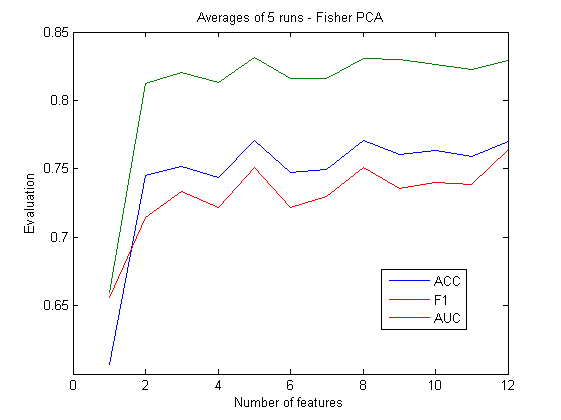
\includegraphics[scale= 0.5]{fisher_pca.png}
		\caption{Fisher PCA}
		\label{fig:minipage1}
	\end{minipage}
	\quad	
	\begin{minipage}[b]{0.45\linewidth}
		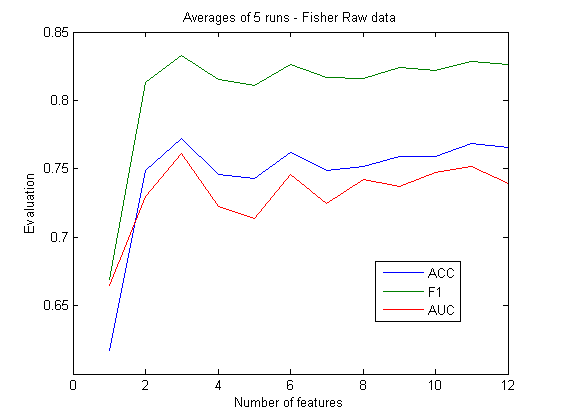
\includegraphics[scale= 0.5]{fisher_raw_data.png}
		\caption{Fisher RAW data}
		\label{fig:minipage2}
	\end{minipage}
\end{figure}

\tab First we calculated the average of 5 runs of fisher, after applying to the dataset the PCA method.\smallskip\\
\tab By looking at the graphic we conclude which has the best number of features for this method. That was 5 features which we can get the F1 value around 0,84 with a accuracy of around 0,76 and the area under the curve was about 0,75.\smallskip\\
\tab After making an average of 5 runs of fisher, with raw data, we got the graphic with accuracy, area under curve and F1.\smallskip\\
\tab By analyses of the graphic, we can see the best values we got was with 3 features, giving F1 values within 0,8 and 0,85, with around 0,77 accuracy and AUC slightly over 0,75.\smallskip\\
\tab When we compare the two methods we can conclude that less of 5 features for PCA data or 3 features with raw data we got very bad results because we had limited information, more of that number of features the results undergo little change, because by increasing the amount of information also increases the complexity of the problem and can take the decision-making capacity.\smallskip\\

\pagebreak
\subsection{k-NN}
\tab Knn is a simple classifier. It consists in choosing the class which is more present in the K samples near the pattern to be tested. By that we mean that analyzing the features dimensionality we get the K trained samples more similar to the one being tested and choose the class which is more present in that k samples.\smallskip\\

\begin{figure}[H]
	\centering
	\begin{minipage}[b]{0.45\linewidth}
		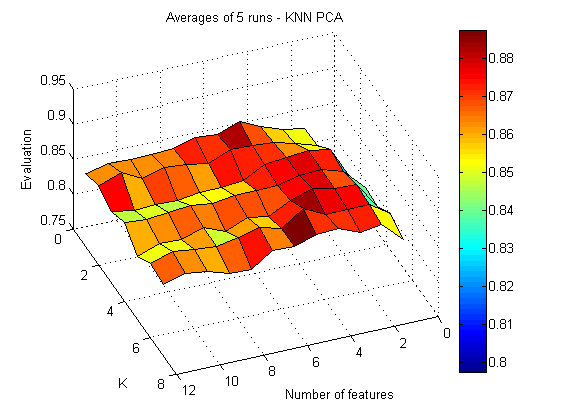
\includegraphics[scale= 0.5]{knn_pca.png}
		\caption{k-NN PCA}
		\label{fig:minipage1}
	\end{minipage}
	\quad	
	\begin{minipage}[b]{0.45\linewidth}
		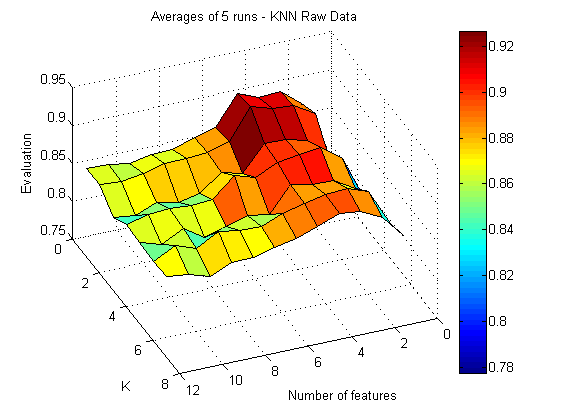
\includegraphics[scale= 0.5]{knn_raw_data.png}
		\caption{k-NN RAW data}
		\label{fig:minipage2}
	\end{minipage}
\end{figure}

\tab After making 5 runs for each number of features with raw data and for each value of K varying from 1 to 7, we easily verify that the best results of F1 score were achieved by K = 2 with 5 features.\smallskip\\
\tab Using PCA the results were not so good.\smallskip\\
\tab It’s interesting how this simple classifier can achieve one of the best results described along this work.\smallskip\\

\pagebreak
\subsection{SVM}
\tab Support Vector machines are machine learning algorithms that intend to answer the question "What is the best separation hyper plane between the two classes?"\smallskip\\
\tab It calculates the hyper plane with the highest margin of separation between classes.\smallskip\\
\tab SVM algorithms base idea is to perform the empirical risk minimization, but not forgetting the structure. This allows such classifiers not to over fit like the classical neural networks since they are aware of the structure.
\begin{figure}[H]
	\centering
	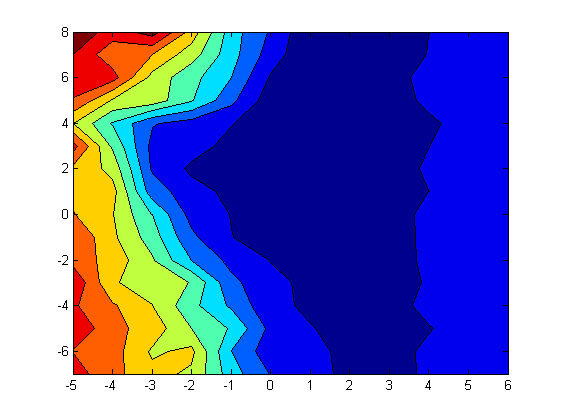
\includegraphics[scale= 0.5]{svm_parameter.png}
	\caption{SVM}
\end{figure}
\tab For SVM we used the rbf kernel.\smallskip\\
\tab We made the parameters vary along the window presented above. For each value of these parameters we built a new training set and testing set and tested SVM classifiers.\smallskip\\
\tab After 5 runs we calculate the averages of the errors and build the upper image in which we can see that the best parameters are near the center of it. We can’t see by the colors, but the best values were 1,4.
\begin{figure}[H]
	\centering
	\begin{minipage}[b]{0.45\linewidth}
		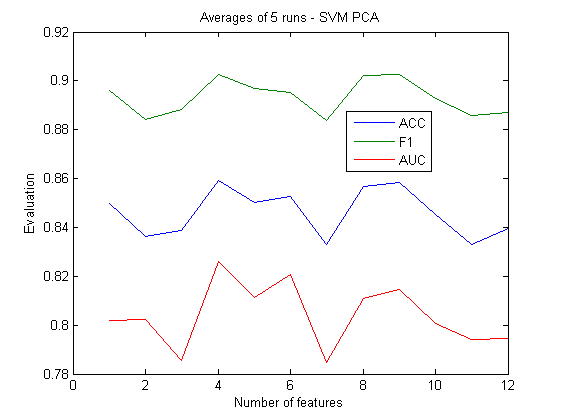
\includegraphics[scale= 0.5]{svm_pca.png}
		\caption{SVM PCA}	
		\label{fig:minipage1}
	\end{minipage}
	\quad	
	\begin{minipage}[b]{0.45\linewidth}
		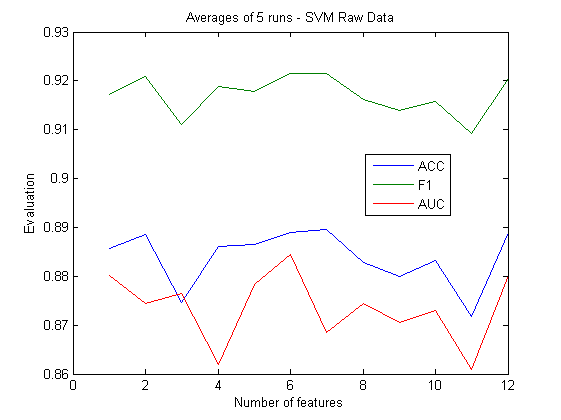
\includegraphics[scale= 0.5]{svm_raw_data.png}
		\caption{SVM Raw data}
		\label{fig:minipage2}
	\end{minipage}	
\end{figure}

\tab So after knowing that the best parameters for SVM were (1,4), we built that classifier with 80\% training, 20\% testing and got the results above for raw data and PCA features.\smallskip\\
\tab In the raw data plot we can see that the results achieved with the SVM classifier were the best results of this work. The F1 varied from 0,91 to 0,92 and the accuracy was in average 0,88 to 0,89. The optimal number of features was 6.\smallskip\\
\tab Using PCA the results were not as good as with the raw data and the optimal number of features was 4.\smallskip\\
\section{Classifier Performance Metrics}
\tab In this step it is important to analyse the performance of the techniques implemented using reliable techniques, we need to have a solid classifier that has good results, and low variability in its performance independent of the dataset used. It is important to use different metrics, most of the times the accuracy of the classifier
is not a good measure. For the sake of having a robust classifier this we are going to use the F1-Score, AUC, Precision and Recall as a complementary techniques to evaluate the classifiers.
\subsection{Accuracy}
\tab The accuracy can be considered the tolerance area of the results, in other words the accuracy consists in the positive results of our system over the total of results.\\
\tab Only using the accuracy as a classifier performance metric is not enough since we could have a classifier that for instance classifies correctly all the confusion matrix correctly except the True Positives and such algorithm could have a good accuracy and still missing all of the important positive matches.
\subsection{F1 Score}
\tab The F1 Score is a measure of the classifier's performance that considers the precision and the recall.Despite being well known in the machine learning subject it is not the best metric to evaluate a binary classifier since it does not take the true negative rate into account.\\
\tab We calculated F1 score using the following formula: F1 = 2TP /(2TP+FP+FN)
\subsection{AUC}
\tab This parameter analysis the classifier's performance using ROC curves, and is the value corresponding to the area under the curve (AUC).\\
\tab When using normalized units, the area AUC is equal to the probability that a classifier will rank a randomly chosen positive instance higher than a randomly chosen negative one.
A reliable and valid AUC metric can be interpreted as the probability that the classifier will assign a higher score to a randomly chosen positive example than to a randomly chosen negative example.
\subsection{Precision}
\tab The precision of a measurement system is the degree to which repeated measurements under unchanged conditions show the same results. This parameter is defined as the proportion of the true positives against all the positive results.
\subsection{Recall}
\tab Recall is the fraction of relevant instances that are retrieved. A high recall means that an algorithm returned most of the relevant results. Recall is defined as the number of true positives divided by the total number of elements that actually belong to the positive class.
\section{Graphical User Interface (GUI)}
\tab In order to present the machine learning methods to the user we created a GUI that allows the user to choose the different options to test and check the performance metrics of the classifier.
\begin{figure}[H]
	\centering
	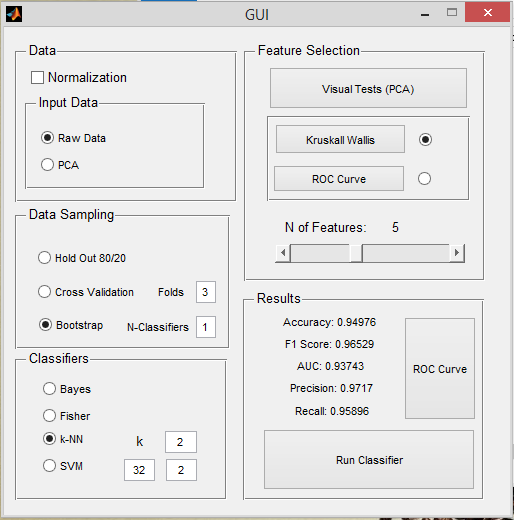
\includegraphics[scale= 0.8]{interface.png}
	\caption{Graphical User Interface}
\end{figure}
\tab In the data separator we define if we are going to use the data as it comes from the Python script, if we are going to normalize it or if we intend to use PCA to project the data.\\
\tab In the Feature selection panel we have implemented multiple tests such as Scree Test, Kaiser Test, Visual Threshold, Kruskall Wallis and ROC curves. Our intent with this options is that the user analyse the information and define how many features to use. Note that the features that are going to be used are the best N features according to the chosen test.\\
\tab The data sampling panel is used to define the method of data sampling used to evaluate the classifier varying from hold-out, cross-validation and bootstrap.\\
\tab As classifiers, we implemented Bayes, Fisher, k-NN in which the user can define the number of k nearest patters and SVMs in which the user can define the C and Gamma parameters.\\
\tab Finally, in the results panel we show the performance metrics of the classifier when using the definitions chosen by the user and it's ROC curve.
\pagebreak
\section{Conclusion}
\tab With this work we learned how to pick a real dataset and extract different features. After having the different features of the dataset we made the selection of the most relevant methods through the Kruskal-Walis, Scree Test and Kaiser Test and AUC. The techniques that revealed more reliability in the final classifier were the Kruskall-Wallis and the ROC-Curves.\\
\tab After choosing the features we analysed diverse data sampling techniques. Here the one that showed better results was the 'simple error bootstrap', since this technique uses all the dataset as input for the tests in all the classifiers. However it is not as reliable as Cross-validation since the test dataset is not independent of the training set. The cross-validation technique also showed high results and low variance.\\
\tab Finally we applied different classifiers to analyse our data, and we get better results with the SVM classifier using 6 features and raw data and bootstrap. With it we obtained the following results: F1 with values of 0,96, with accuracy around 0.95, and an area under the curve around 0,93.\\
\tab On the other hand we have the k-NN classifier which in turn is a very simple classifier, also obtained very good results, 5 features, raw data, bootstrap: Accuracy 0.94, F1 0.96, AUC 0.93.

%\section{Bibliography}

\end{document}